% Options for packages loaded elsewhere
\PassOptionsToPackage{unicode}{hyperref}
\PassOptionsToPackage{hyphens}{url}
%
\documentclass[
  english,
  man,floatsintext]{apa6}
\usepackage{lmodern}
\usepackage{amssymb,amsmath}
\usepackage{ifxetex,ifluatex}
\ifnum 0\ifxetex 1\fi\ifluatex 1\fi=0 % if pdftex
  \usepackage[T1]{fontenc}
  \usepackage[utf8]{inputenc}
  \usepackage{textcomp} % provide euro and other symbols
\else % if luatex or xetex
  \usepackage{unicode-math}
  \defaultfontfeatures{Scale=MatchLowercase}
  \defaultfontfeatures[\rmfamily]{Ligatures=TeX,Scale=1}
\fi
% Use upquote if available, for straight quotes in verbatim environments
\IfFileExists{upquote.sty}{\usepackage{upquote}}{}
\IfFileExists{microtype.sty}{% use microtype if available
  \usepackage[]{microtype}
  \UseMicrotypeSet[protrusion]{basicmath} % disable protrusion for tt fonts
}{}
\makeatletter
\@ifundefined{KOMAClassName}{% if non-KOMA class
  \IfFileExists{parskip.sty}{%
    \usepackage{parskip}
  }{% else
    \setlength{\parindent}{0pt}
    \setlength{\parskip}{6pt plus 2pt minus 1pt}}
}{% if KOMA class
  \KOMAoptions{parskip=half}}
\makeatother
\usepackage{xcolor}
\IfFileExists{xurl.sty}{\usepackage{xurl}}{} % add URL line breaks if available
\IfFileExists{bookmark.sty}{\usepackage{bookmark}}{\usepackage{hyperref}}
\hypersetup{
  pdftitle={Conceptual Replication of ``Compatibility between Physical Stimulus Size and Left-right Responses: Small is Left and Large is Right''},
  pdfauthor={Alexander Prochnow, Paul Jänsch, Pia Stermann and Ludger Masch},
  pdflang={en-EN},
  pdfkeywords={ATOM; compatibility; stimulus size; response location},
  hidelinks,
  pdfcreator={LaTeX via pandoc}}
\urlstyle{same} % disable monospaced font for URLs
\usepackage{graphicx,grffile}
\makeatletter
\def\maxwidth{\ifdim\Gin@nat@width>\linewidth\linewidth\else\Gin@nat@width\fi}
\def\maxheight{\ifdim\Gin@nat@height>\textheight\textheight\else\Gin@nat@height\fi}
\makeatother
% Scale images if necessary, so that they will not overflow the page
% margins by default, and it is still possible to overwrite the defaults
% using explicit options in \includegraphics[width, height, ...]{}
\setkeys{Gin}{width=\maxwidth,height=\maxheight,keepaspectratio}
% Set default figure placement to htbp
\makeatletter
\def\fps@figure{htbp}
\makeatother
\setlength{\emergencystretch}{3em} % prevent overfull lines
\providecommand{\tightlist}{%
  \setlength{\itemsep}{0pt}\setlength{\parskip}{0pt}}
\setcounter{secnumdepth}{-\maxdimen} % remove section numbering
% Make \paragraph and \subparagraph free-standing
\ifx\paragraph\undefined\else
  \let\oldparagraph\paragraph
  \renewcommand{\paragraph}[1]{\oldparagraph{#1}\mbox{}}
\fi
\ifx\subparagraph\undefined\else
  \let\oldsubparagraph\subparagraph
  \renewcommand{\subparagraph}[1]{\oldsubparagraph{#1}\mbox{}}
\fi
% Manuscript styling
\usepackage{upgreek}
\captionsetup{font=singlespacing,justification=justified}

% Table formatting
\usepackage{longtable}
\usepackage{lscape}
% \usepackage[counterclockwise]{rotating}   % Landscape page setup for large tables
\usepackage{multirow}		% Table styling
\usepackage{tabularx}		% Control Column width
\usepackage[flushleft]{threeparttable}	% Allows for three part tables with a specified notes section
\usepackage{threeparttablex}            % Lets threeparttable work with longtable

% Create new environments so endfloat can handle them
% \newenvironment{ltable}
%   {\begin{landscape}\begin{center}\begin{threeparttable}}
%   {\end{threeparttable}\end{center}\end{landscape}}
\newenvironment{lltable}{\begin{landscape}\begin{center}\begin{ThreePartTable}}{\end{ThreePartTable}\end{center}\end{landscape}}

% Enables adjusting longtable caption width to table width
% Solution found at http://golatex.de/longtable-mit-caption-so-breit-wie-die-tabelle-t15767.html
\makeatletter
\newcommand\LastLTentrywidth{1em}
\newlength\longtablewidth
\setlength{\longtablewidth}{1in}
\newcommand{\getlongtablewidth}{\begingroup \ifcsname LT@\roman{LT@tables}\endcsname \global\longtablewidth=0pt \renewcommand{\LT@entry}[2]{\global\advance\longtablewidth by ##2\relax\gdef\LastLTentrywidth{##2}}\@nameuse{LT@\roman{LT@tables}} \fi \endgroup}

% \setlength{\parindent}{0.5in}
% \setlength{\parskip}{0pt plus 0pt minus 0pt}

% \usepackage{etoolbox}
\makeatletter
\patchcmd{\HyOrg@maketitle}
  {\section{\normalfont\normalsize\abstractname}}
  {\section*{\normalfont\normalsize\abstractname}}
  {}{\typeout{Failed to patch abstract.}}
\patchcmd{\HyOrg@maketitle}
  {\section{\protect\normalfont{\@title}}}
  {\section*{\protect\normalfont{\@title}}}
  {}{\typeout{Failed to patch title.}}
\makeatother
\shorttitle{Conceptual Replication}
\keywords{ATOM; compatibility; stimulus size; response location\newline\indent Word count: X}
\DeclareDelayedFloatFlavor{ThreePartTable}{table}
\DeclareDelayedFloatFlavor{lltable}{table}
\DeclareDelayedFloatFlavor*{longtable}{table}
\makeatletter
\renewcommand{\efloat@iwrite}[1]{\immediate\expandafter\protected@write\csname efloat@post#1\endcsname{}}
\makeatother
\usepackage{csquotes}
\usepackage[titles]{tocloft}
\cftpagenumbersoff{figure}
\renewcommand{\cftfigpresnum}{\itshape\figurename\enspace}
\renewcommand{\cftfigaftersnum}{.\space}
\setlength{\cftfigindent}{0pt}
\setlength{\cftafterloftitleskip}{0pt}
\settowidth{\cftfignumwidth}{Figure 10.\qquad}
\cftpagenumbersoff{table}
\renewcommand{\cfttabpresnum}{\itshape\tablename\enspace}
\renewcommand{\cfttabaftersnum}{.\space}
\setlength{\cfttabindent}{0pt}
\setlength{\cftafterloftitleskip}{0pt}
\settowidth{\cfttabnumwidth}{Table 10.\qquad}
\ifxetex
  % Load polyglossia as late as possible: uses bidi with RTL langages (e.g. Hebrew, Arabic)
  \usepackage{polyglossia}
  \setmainlanguage[]{english}
\else
  \usepackage[shorthands=off,main=english]{babel}
\fi

\title{Conceptual Replication of ``Compatibility between Physical Stimulus Size and Left-right Responses: Small is Left and Large is Right''}
\author{Alexander Prochnow, Paul Jänsch, Pia Stermann and Ludger Masch\textsuperscript{}}
\date{}


\authornote{

Add complete departmental affiliations for each author here. Each new line herein must be indented, like this line.

Enter author note here.

The authors made the following contributions. Alexander Prochnow, Paul Jänsch, Pia Stermann and Ludger Masch: Conceptualization, Writing - Original Draft Preparation, Writing - Review \& Editing.

Correspondence concerning this article should be addressed to Alexander Prochnow, Paul Jänsch, Pia Stermann and Ludger Masch, Postal address. E-mail: \href{mailto:my@email.com}{\nolinkurl{my@email.com}}

}

\affiliation{\vspace{0.5cm}\textsuperscript{} University of Osnabrück}

\abstract{
One or two sentences providing a \textbf{basic introduction} to the field, comprehensible to a scientist in any discipline.

Two to three sentences of \textbf{more detailed background}, comprehensible to scientists in related disciplines.

One sentence clearly stating the \textbf{general problem} being addressed by this particular study.

One sentence summarizing the main result (with the words ``\textbf{here we show}'' or their equivalent).

Two or three sentences explaining what the \textbf{main result} reveals in direct comparison to what was thought to be the case previously, or how the main result adds to previous knowledge.

One or two sentences to put the results into a more \textbf{general context}.

Two or three sentences to provide a \textbf{broader perspective}, readily comprehensible to a scientist in any discipline.
}



\begin{document}
\maketitle

ATOM (\enquote{A theory of magnitude}) is a theory proposed by Walsh(2003), which basically assumes a generalized magnitude-processing system in the brain where relations between the cortical representations of \enquote{time, space and quantity} exist. The theory predicts that if there were such relations then there must be interference and congruency effects in experimental research investigating stimulus-response tendencies comprising different numerical, temporal or spatial properties.
Many studies have investigated different aspects and proposals of this theory in terms of Stimulus-response (S-R) compatibility, where S-R compatibility refers to how \enquote{natural} it is for a certain required response (or action) to follow a given stimulus type. Typically, such compatibility effects are investigated by comparing reaction times for a required action or response in experimental tasks with a specifically defined Stimulus-Response mapping that is varied within the experiment. For example Dehaene et al.(1990) found compatibility effects between numerical size and horizontal response location, which Dehaene et al.(1993) later coined as \enquote{Spatial-Numerical Association of Response Codes} (SNARC) effect. The SNARC effect is interpreted as a spatial mapping of numbers to horizontal locations.
In 2013, Ren et al.~have furthermore analogously investigated the relationship between physical stimulus size and horizontal response location. Their results show similar compatibility effects of stimulus size and horizontal response location, but only for right hand responses. In 2018, Wühr and Seegelke attempted a conceptual replication and extension of this study. They claim that their results indicate the existence of a general magnitude code, as proposed in ATOM in that we might intrinsically associate small objects with the left side and large objects with the right.
In the experiment, subjects are presented with \enquote{small} or \enquote{large} stimulus objects (squares) and are required to judge their size as \enquote{small} or \enquote{large}. The keys for subjects to communicate these judgements are mapped to either left- or right-hand responses and these mappings are switched once within the experiment. Wühr and Seegelke(2018) found, that participants were faster to respond to a large stimulus object with a key that is on the right of the keyboard (e.g.~\enquote{Backspace}, pressed with the right hand), than with a key that is on the left of the keyboard (e.g.~\enquote{Tabulator}, pressed with the left hand). For small stimulus objects, they found that reaction times were numerically faster for left-hand responses than for right-hand responses.
For participants to judge whether the stimulus is a small or large object, ATOM would propose that subjects need to mentally activate an internal representation of size and the corresponding spatial response mapping in order to generate an action as response according to their judgement about stimulus size, and that these representations are linked. Ren et al.~(2011), and Wühr and Seegelke (2018) showed that stimulus size and horizontal response location indeed exhibit compatibility effects, which can be regarded as evidence for this sub-aspect of ATOM. They found that the horizontal response mapping (key press with either left or right hand) to judgements about stimuli of different size influences response behavior and matters for success and swiftness of judgements of \enquote{small} or \enquote{large} stimulus objects.
We here aimed to assess the findings of Wühr and Segeelke(2018) via a conceptual replication of the first experiment and extended it by not only taking right-handed participants into account but also seperately testing left-handed participants. Our hypotheses were based on their results that small stimuli are associated with left-hand responses, whereas large stimuli are associated with right-hand responses. We sought to replicate similar stimulus size - response location compatibility effects as those reported by Wühr and Segeelke(2018), that means we wanted to find out whether different stimulus-response mapping conditions have an effect on participant's reaction time to a specific type of stimulus (in this case large or small square). Additionally we aimed to investigate whether we can find compatibility effects in opposite direction for left-handed participants. However we changed
In particular we tested for right-handed participants if response times for right-hand responses are faster to the larger stimulus than to the smaller stimulus and similarly if response times for left-hand responses are faster to the smaller stimulus than to the larger stimulus. Furthermore we investigated if the stimulus size -- response location compatibility effect is larger for right-hand responses than for left-hand responses. This would mean that the difference in response times for right-hand responses to be faster to the larger stimulus than to the smaller stimulus is larger than the difference in response times for left-hand responses to be faster to the smaller stimulus than to the larger stimulus.
Correspondingly we tested the former hypotheses in the opposite direction for left-handed participants. In other words we assumed that the response times for left-hand responses are faster to the larger stimulus than to the smaller stimulus as well as that the response times for right-hand responses are faster to the smaller stimulus than to the larger stimulus. Analogously we hypothesized that here the stimulus size - response location compatibility effect will be larger for the left-hand responses instead of right-hand responses. In the end we compared the size of possible compatibility effects regarding people's handedness and assumed that the stimulus size- response location compatibility effect is larger for right-handed people than for left-handed people. I.e., the absolute difference between response times in the compatible condition and response times in the incompatible condition is larger for right-handed than for left-handed people.

\hypertarget{methods}{%
\section{Methods}\label{methods}}

We report how we determined our sample size, all data exclusions (if any), all manipulations, and all measures in the study.

\hypertarget{participants}{%
\subsection{Participants}\label{participants}}

We recruited N = 72 participants (43 woman, 27 men, 2 others, 22.60 = mean, age range: 14-55 years) by distributing the link to the experiment via social media, mainly WhatsApp, Facebook and Reddit (see Table 1 for demographics). The link was hosted on Netlify (citation). 59 of the participants were right-handed and 12 were left-handed, as well as 1 participant indicating mixed-handedness. They were advised to take part only once, however, we did not control for this. On average, participants needed 12.89 minutes to complete the experiment, with a minimum time of 9.84 minutes and a maximum time of 21.07 minutes after filtering (explained in the data preparation section). The link was available for four days until we closed collection of data (from the 31st of July 2020 until the 3rd of August 2020). Before taking part, the participants declared to have normal or corrected-to-normal visual acuity and should be naive with respect to the purpose of the study. Participation was voluntary and not rewarded with money or material things but with our deep gratitude.

\hypertarget{material}{%
\subsection{Material}\label{material}}

In each trial, a visual stimulus object was presented in the center of the screen with white background. A stimulus object in the experimental block was a simple black square, which was either small (about 3 x 3 cm, depending on the size of the screen) or large (edges twice as long as those of the small stimulus, i.e.~about 6 x 6 cm, depending on the size of the screen). We used information about the stimulus objects (i.e.~information about how they are to be displayed concerning their form, size and position on the display) as provided by Wühr and Seegelke (2018), however we could not guarantee an exact same formatting of stimuli for each participant in terms of equal edge lengths, but only in terms of relations between edge lengths, since the size of the displayed stimulus was relative to the screen on which it was presented. The 2 different types of stimulus objects were used for training trials and main trials in both experimental blocks. Additionally to the original study we included an intermediate block which was intended as a distraction. A stimulus object in this block was either a simple black circle or a simple black triangle, both of small to intermediate size - regarding the small and large square stimulus objects' edge lengths- in terms of the circle's diameter or the triangle's height.
~

\hypertarget{procedure}{%
\subsection{Procedure}\label{procedure}}

The experiment consisted of 10 parts. These parts comprised the two main experimental blocks, one for each of the two S-R mapping conditions, and one intermediate block with the distraction tasks. We varied the stimulus size - response (key) location mapping (S-R mapping) for the experimental blocks once over the course of the experiment. The order of S-R mapping conditions for the first and second experimental blocks (first = compatible -- second = incompatible or first = incompatible -- second = compatible) was determined experiment initially, uniformly at random once for each participant. In the compatible mapping condition, the small stimulus required a response with the left (\enquote{q}) key, whereas the large stimulus required a response with the right (\enquote{p}) key. The mapping was reversed in the incompatible mapping condition.
At the beginning of the experiment, participants were welcomed and given (not further specified) information about the general procedure, namely, that the experiment will consist of several parts, which again consist of several trials of tasks of similar structure. It was recommended to the participants to complete the whole experiment (to prevent dropouts from the beginning on), and they were given information about the approximate duration of the experiment (about 15 minutes).
More precise descriptions of the participant's task were presented at the beginning of each block. These specific instructions included information about the sequence of events in a trial (fixation - stimulus presentation - key press or button click given the assigned S-R mapping), i.e.~which keys to press for \enquote{small} or \enquote{large} stimuli (corresponding to the respective S-R mapping condition) in the experimental task blocks, or which buttons to click on for \enquote{circle} or \enquote{triangle} in the distracting task block, as well as information on whether the next part belongs to training (for the experimental blocks) or experimental phase (as in the intermediate block). Additionally, all instructions emphasized that participants should strive to optimize speed and accuracy (this was not mentioned in the original paper but seemed appropriate in this context, since a time-out occurred and an error message was displayed after the key press when participants' response time(RT) exceeded a period of 2000 ms).
After having read the initial instructions of a new experimental block, participants firstly performed a training trial phase (10 trials) before they proceeded with the main experimental trial phase for the respective S-R mapping condition(2 stimuli × 30 repetitions = 60 trials). The first experimental block was followed by written instructions about the intermediate task, in which participants were shown either a circle or a triangle and had to classify the presented stimulus as \enquote{circle} or \enquote{triangle} by clicking on the respective button at the bottom of the screen. The intermediate task had (2 stimuli × 10 repetitions =) 20 main trials. The specific number of the intermediate task's trials was not necessarily optimal, but we decided on this as a -hopefully well - balanced compromise between effective distraction and no unnecessary prolonging of the experiment. The order in which participants were shown either of the two stimuli in the intermediate task was determined uniformly at random. After completion of the intermediate block's trials, participants were shown written instructions of the following experimental block (similar to the initial experimental block's instructions, only different in the description of the S-R mapping, since it was reversed here). They then performed a training block (10 trials) and an experimental block with the respective second S-R mapping (2 stimuli × 30 repetitions).
During the training phases participants accustomed to the task, specifically to the respective S-R mapping, by completing the given amount of practice trials. Practice trials differed from main trials in that participants received a short feedback message, telling them whether their answer was correct (namely: \enquote{Correct!} or \enquote{Incorrect!}).
The order in which individual trials are presented in the training and experimental phases is determined uniformly at random and on the fly for each participant.
All experimental trials were structured as follows. Each trial started with the presentation of a fixation point (a small black \enquote{x} sign) for 1000 ms in the center of the screen. Afterwards one of the two stimulus objects were displayed until a keypress (experimental blocks) or button click (intermediate block) occurred. In the experimental blocks, participants responded by pressing the left \enquote{q} key or the right \enquote{p} key on their keyboard. Participants should operate the left key (\enquote{q}) with the index finger of their left hand and the right key (\enquote{p}) with the index finger of their right hand. In the intermediate task, participants responded by clicking on the \enquote{circle} or \enquote{triangle} button at the bottom the screen. A correct response with a response time below 2000 ms after stimulus presentation was followed by a blank screen for 1500 ms. If the \enquote{q} or the \enquote{p} key was pressed after the maximum response period of 2000 ms, a corresponding error message (precisely: \enquote{Try to respond more quickly!}) was shown for 1500 ms in black color. In the intermediate block however each of the trials had to be initiated by clicking on a \enquote{start} button in the middle of the screen. In the main experimental blocks the next trial started automatically after the \enquote{p} or \enquote{q} key was pressed. Finally, the experiment terminated with a post-experiment survey asking participants for their preferred handedness (participants could choose between \enquote{right-handed} (default option), \enquote{left-handed} and \enquote{no preference}) and to optionally supply socio-demographic information (age, gender, level of education, native languages, whether there were any technical issues experienced during the experiment). Participants were able to leave comments on the experiment by entering them in a text field.

\hypertarget{data-preparation}{%
\subsection{Data Preparation}\label{data-preparation}}

Originally, our data contained 3 participants who needed drastically longer for the experiment than the average participant. We filtered out these 3 participants by choosing a threshold of 25 minutes, which these participants were well above. Figure X shows our rationale for choosing the threshold quite clearly, as these three participants likely took a break during the experiment or performed another activity, which was not intended by our experimental design. This additional data exclusion criterion was not stated in our preregistration report, because we had not forseen this unintended effect of conducting an online experiment, however the longer break in between trial blocks might cause those participants to perform differently in the following trials. To be on the safe side we therefore excluded these participant's data from our analyses.

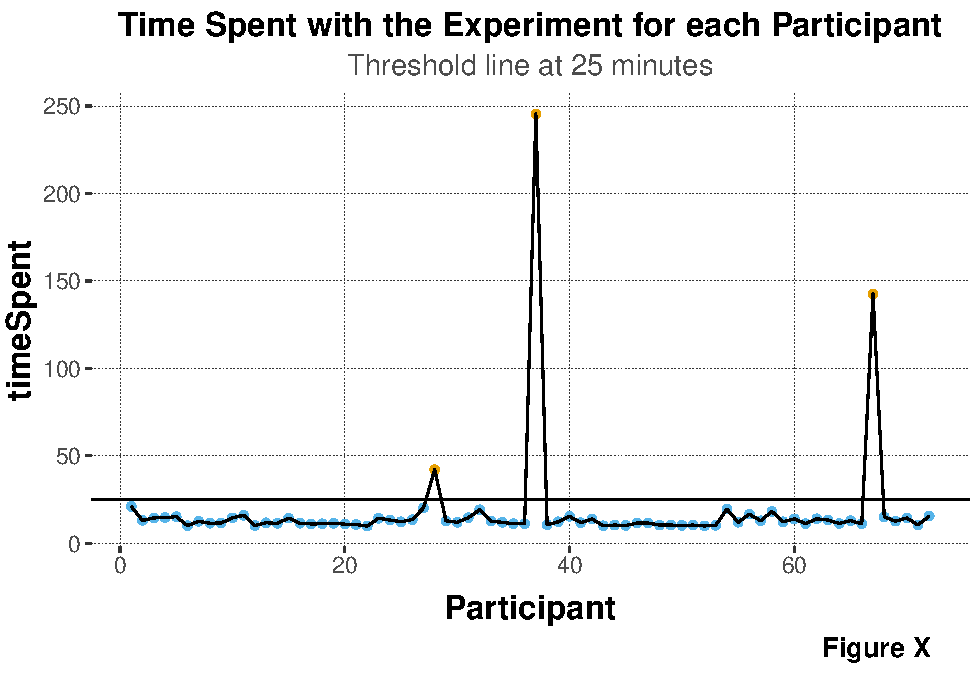
\includegraphics{APA_Template_files/figure-latex/unnamed-chunk-4-1.pdf}

Additionally, we filtered out 1 mixed-handed participant, since their data does not fit into our hypotheses, however we wanted to include the option in our post-experiment survey to not classify data incorrectly. We made this decision after submitting the preregistration report, but think this exclusion follows naturally from our hypotheses, since they only specify to use data from either left- or right-handed participants or both.

\hypertarget{data-analysis}{%
\subsection{Data analysis}\label{data-analysis}}

We used R (Version 4.0.0; R Core Team, 2020) and the R-package \emph{papaja} (Version 0.1.0.9997; Aust \& Barth, 2020) for all our analyses.

\hypertarget{results}{%
\section{Results}\label{results}}

\hypertarget{discussion}{%
\section{Discussion}\label{discussion}}

\newpage

\hypertarget{references}{%
\section{References}\label{references}}

\begingroup
\setlength{\parindent}{-0.5in}
\setlength{\leftskip}{0.5in}

\hypertarget{refs}{}
\leavevmode\hypertarget{ref-R-papaja}{}%
Aust, F., \& Barth, M. (2020). \emph{papaja: Create APA manuscripts with R Markdown}. Retrieved from \url{https://github.com/crsh/papaja}

\leavevmode\hypertarget{ref-R-base}{}%
R Core Team. (2020). \emph{R: A language and environment for statistical computing}. Vienna, Austria: R Foundation for Statistical Computing. Retrieved from \url{https://www.R-project.org/}

\endgroup


\clearpage
\renewcommand{\listfigurename}{Figure captions}

\clearpage
\renewcommand{\listtablename}{Table captions}


\end{document}
